\section{Auswertung}
\subsection{Justierung}
Als grobe Näherung der Resonanzfrequenz des festen Schwingkreises wurden $35,21Hz$ gemessen.

\subsection{Frequenzverhältnisse bei einer Schwebung}
\label{sec:Frequenzverhältnisse}
Diese Messreihe wurde bei einer Generatorfrequenz von ca. $600Hz$ durchgeführt.
Die gezählten Verhältnisse der Frequenzen lassen sich Tabelle \ref{tab:verhaeltnisse} entnehmen. Da die Grenzen der Schwebung nicht immer eindeutig ab zu lesen sind, wird eine Abweichung von $\pm1$ veranschlagt. Graphisch ergibt sich so Abb. \ref{fig:verhaeltnisse}, wobei $\omega_\pm=v_+ \pm v_-$ gilt und $C_k$ mit $3\%$ Abweichung behaftet ist.

\begin{table}
  \centering
\caption{gemessene Frequenzverhältnisse}
\label{tab:verhaeltnisse}
\sisetup{round-mode = places , round-precision = 2}
\begin{tabular}{S S}
  \toprule
  {$C_k/nF$} & {Peaks pro Schwebung}\\
  \midrule
  12.00000000000000000 & 17.00000000000000000\\
  9.990000000000000213e+00 & 14.00000000000000000\\
  8.179999999999999716e+00 & 13.00000000000000000e+00\\
  6.860000000000000320e+00 & 10.00000000000000000e+00\\
  4.740000000000000213e+00 & 9.000000000000000000e+00\\
  2.859999999999999876e+00 & 5.000000000000000000e+00\\
  2.189999999999999947e+00 & 4.000000000000000000e+00\\
\bottomrule
\end{tabular}
\end{table}
\FloatBarrier

\begin{figure}
  \centering
  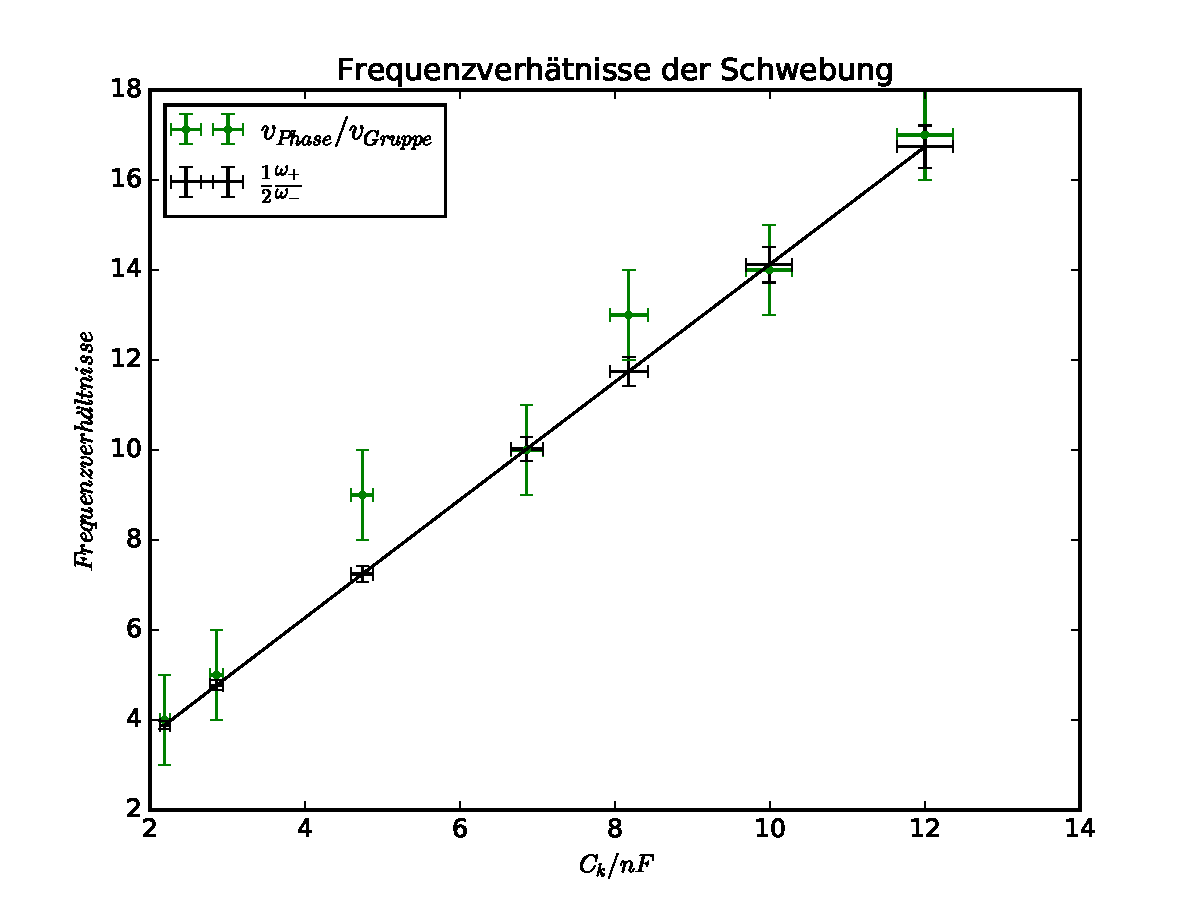
\includegraphics[width=\textwidth]{./plots/freq-ratio.pdf}
  \caption{gezählte Peaks pro Schwebung aufgetragen gegen $C_K$  und vergleichende Theoriegerade}
  \label{fig:verhaeltnisse}
\end{figure}
\FloatBarrier

\subsection{Messung von $v_+$ und $v_-$ mittels Lissajous-Figuren}
\label{sec:Messung-v}


\begin{figure}
  \centering
  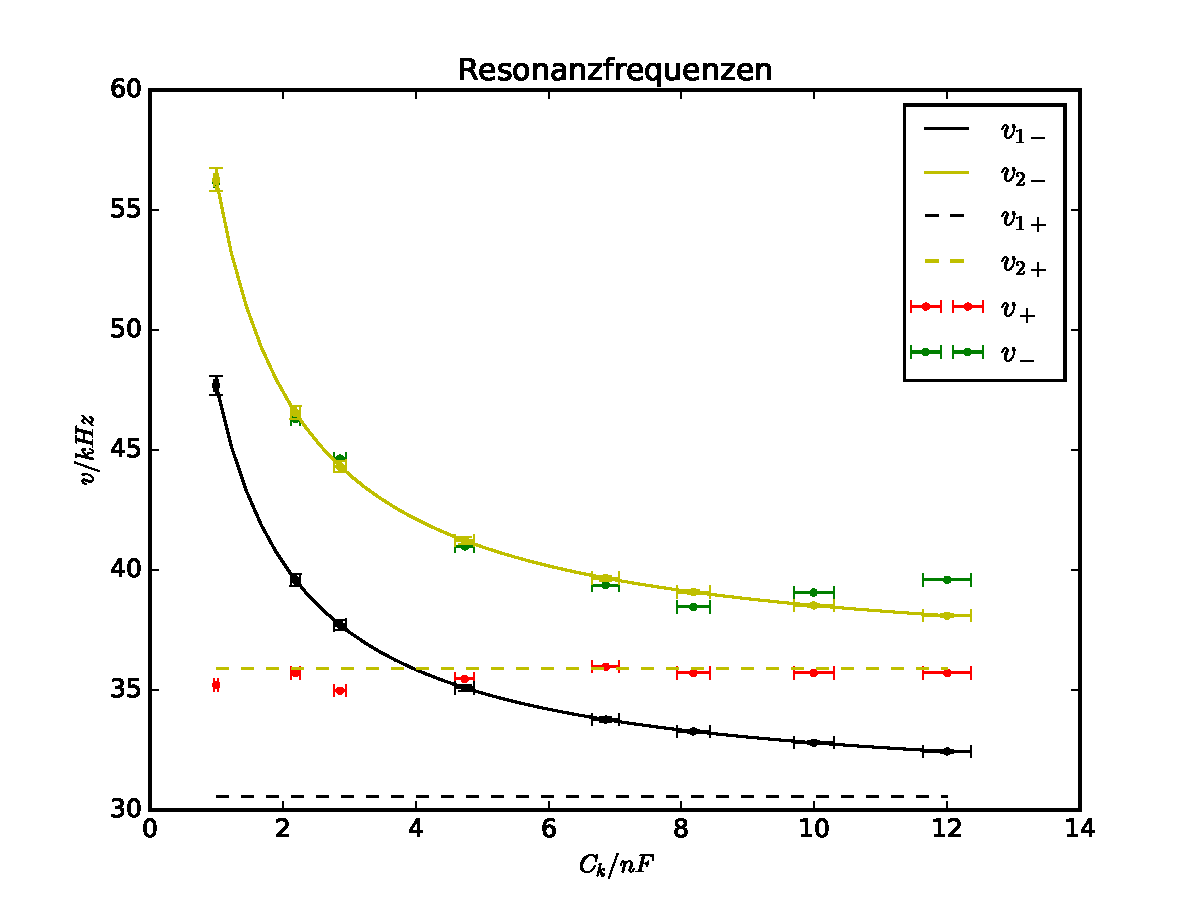
\includegraphics[width=\textwidth]{./plots/resonance.pdf}
  \caption{$v_+$ und $v_-$ aufgetragen gegen $C_K$.}
  \label{fig:frequenzen}
\end{figure}
\FloatBarrier

Die in diesem Schritt aufgenommenen Werte werden in Abb.\ref{fig:frequenzen} mit errechneten Kurven $v_{1-}$ und $v_{2-}$ für Schaltung 1 und 2 aufgetragen. Offensichtlich wurde Schaltung 2 für die Messungen verwendet, weshalb fortan ausschließlich diese Schaltung betrachtet wird. Die Theorie-Kurven ergeben sich hierbei aus den Formeln \eqref{eqn:nu+} und \eqref{eqn:nu-}.

\begin{table}
  \centering
\caption{gemessene Resonanzfrequenzen}
\label{tab:verhaeltnisse}
\sisetup{round-mode = places , round-precision = 2}
\begin{tabular}{S S S}
  \toprule
  {$C_k/nF$} & {$v_+/kHz$} & {$v_-/kHz$}\\
  \midrule
  0.9969999999999999973e-00 & 35.20000000000000284e+00 & 46.29999999999999716e+00\\
  2.189999999999999947e+00 & 35.70000000000000284e+00 & 56.17999999999999972e+00\\
  2.859999999999999876e+00 & 34.96999999999999886e+00 & 44.64000000000000057e+00\\
  4.740000000000000213e+00 & 35.46000000000000085e+00 & 40.97999999999999687e+00\\
  6.860000000000000320e+00 & 35.96999999999999886e+00 & 39.36999999999999744e+00\\
  8.179999999999999716e+00 & 35.71000000000000085e+00 & 38.46000000000000085e+00\\
  9.990000000000000213e+00 & 35.71000000000000085e+00 & 39.06000000000000227e+00\\
  12.00000000000000000e+00 & 35.71000000000000085e+00 & 39.59000000000000341e+00\\
\bottomrule
\end{tabular}
\end{table}
\FloatBarrier


\subsection{Ermittlung von $v_+$ und $v_-$ mittels Sweep-Verfahren}
\label{sec:sweep}

Da beim Sweep-Verfahren die Frequenzen nicht direkt gemessen werden, sondern nur zeitliche Abstände (zu entnehmen aus Tabelle \ref{tab:sweep}) müssen diese zunächst umgerechnet werden. Hierzu wird folgende Formel verwendet:

\begin{equation}
  f(t) = ( f_{Ende} - f_{Anfang} ) \frac{t}{1s} + f_{Anfang}
\end{equation}

Bei der Messung sind $f_{Anfang} = 3,165kHz$ und $f_{Ende} = 83,33kHz$ gewählt.

\begin{table}
  \centering
\caption{Zeitdifferenzen der Resonanzfrequenzen beim Sweep}
\label{tab:sweep}
\sisetup{round-mode = places , round-precision = 2}
\begin{tabular}{S S S}
  \toprule
  {$C_k/nF$} & {$\Delta t/ms$} & {$\Delta t/ms$}\\
  \midrule
  0.9969999999999999973e-00 & 400.0000000000000000e+00 & 648.0000000000000000e+00\\
  2.189999999999999947e+00 & 408.0000000000000000e+00 & 536.0000000000000000e+00\\
  2.859999999999999876e+00 & 400.0000000000000000e+00 & 504.0000000000000000e+00\\
  4.40000000000000213e+00 & 408.0000000000000000e+00 & 464.0000000000000000e+00\\
  6.860000000000000320e+00 & 400.0000000000000000e+00 & 440.0000000000000000e+00\\
  8.179999999999999716e+00 & 400.0000000000000000e+00 & 440.0000000000000000e+00\\
  9.990000000000000213e+00 & 408.0000000000000000e+00 & 432.0000000000000000e+00\\
  12.00000000000000000e+00 & 392.0000000000000000e+00 & 416.0000000000000000e+00\\
\bottomrule
\end{tabular}
\end{table}
\FloatBarrier

\begin{table}
  \centering
\caption{Resonanzfrequenzen gemessen mit sweep}
\label{tab:sweep}
\sisetup{round-mode = places , round-precision = 2}
\begin{tabular}{S S S}
  \toprule
  {$C_k/nF$} & {$\frac{v_+}{kHz}$} & {$\frac{v_-}{kHz}$}\\
  \midrule
  0.9969999999999999973e-00 & 35.23100000000000165e+00 & 55.11192000000000490e+00\\
  2.189999999999999947e+00 & 35.87232000000000198e+00 & 46.13344000000000733e+00\\
  2.859999999999999876e+00 & 35.23100000000000165e+00 & 43.56816000000000599e+00\\
  4.740000000000000213e+00 & 35.87232000000000198e+00 & 40.36156000000000432e+00\\
  6.860000000000000320e+00 & 35.23100000000000165e+00 & 38.43760000000000332e+00\\
  8.179999999999999716e+00 & 35.23100000000000165e+00 & 38.43760000000000332e+00\\
  9.990000000000000213e+00 & 35.87232000000000198e+00 & 37.79628000000000299e+00\\
  12.00000000000000000e+00 & 34.58968000000000131e+00 & 36.51364000000000232e+00\\

\bottomrule
\end{tabular}
\end{table}
\FloatBarrier


\begin{figure}
  \centering
  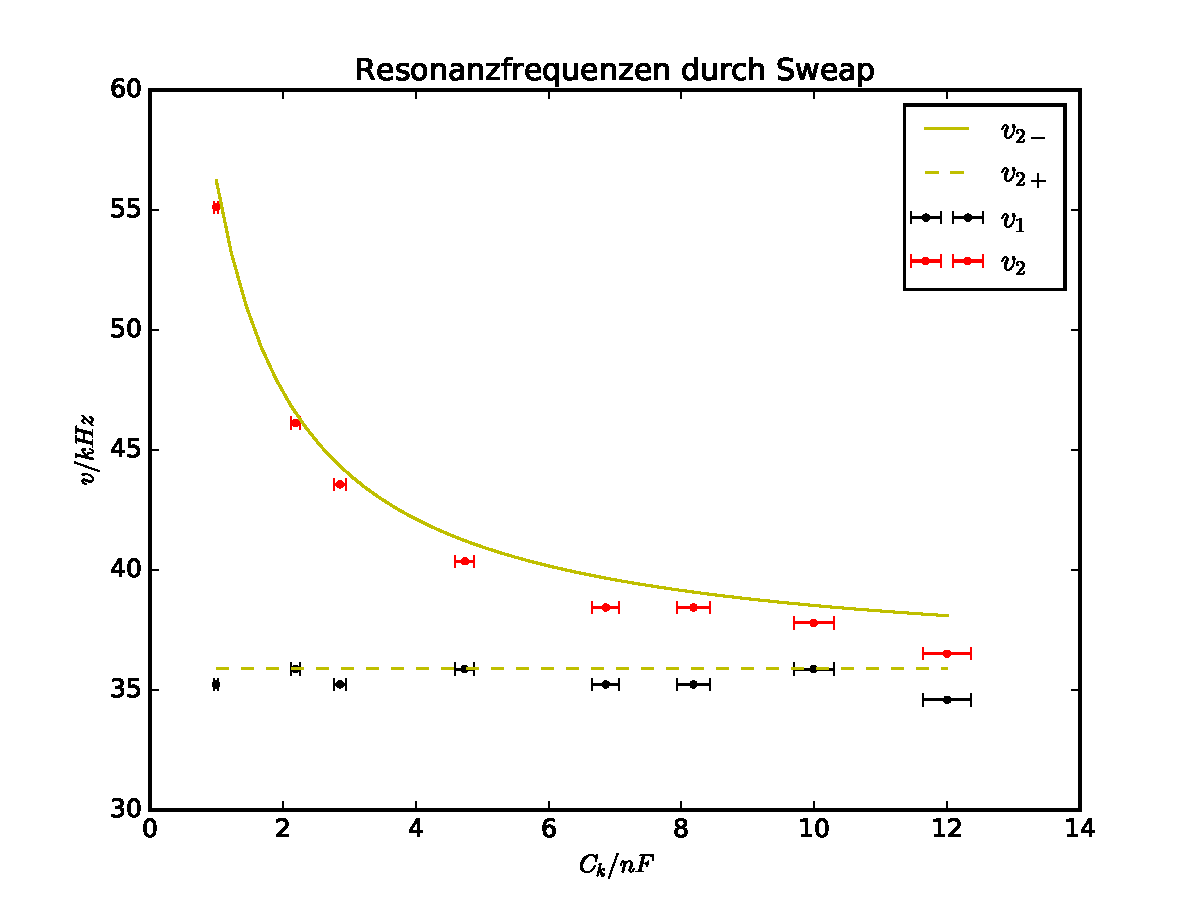
\includegraphics[width=\textwidth]{./plots/sweap.pdf}
  \caption{$v_+$ und $v_-$ aufgetragen gegen $C_K$.}
  \label{fig:sweep}
\end{figure}
\FloatBarrier
